\documentclass[a4paper]{article}

%% Language and font encodings
\usepackage[english]{babel}
\usepackage[utf8x]{inputenc}
\usepackage[T1]{fontenc}

%% Sets page size and margins
\usepackage[a4paper,top=3cm,bottom=2cm,left=3cm,right=3cm,marginparwidth=1.75cm]{geometry}

%% Useful packages
\usepackage{amsmath}
\usepackage{graphicx}
\usepackage[colorinlistoftodos]{todonotes}
\usepackage[colorlinks=true, allcolors=blue]{hyperref}
\usepackage{float}
\usepackage{enumerate}
\usepackage{subfig}
\setlength\parindent{0pt}
\usepackage{amssymb}
\setcounter{section}{-1}
\title{MA 503 : Homework 4+}
\author{Dane Johnson}

\begin{document}
\maketitle




{\bf Problem 40}\\

Let $F$ be a closed set of real numbers and $f$ a real valued function which is defined and continuous on $F$. Show there is a function $g : \mathbb{R}\rightarrow \mathbb{R}$ such that $g$ is continuous and $f(x) = g(x)$ for each $x \in F$. \\

If $F = \emptyset$, use $g(x) \equiv 0$. Then $g$ is continuous and the requirement that $f(x) = g(x)$ for each $x \in F$ is vacuously true.\\

If $F = \mathbb{R}$, then set $g \equiv f$. Since $f$ is continuous $g$ is also continuous on $\mathbb{R}$ and $g(x) = f(x)$ for each $x \in F = \mathbb{R}$. \\

If $F \subsetneq \mathbb{R}$ then $F^c$ is a nonempty open set of real numbers. Using Proposition 8, $F^c$ is the union of a countable collection of disjoint open sets, not all empty. As in the proof of this proposition, for each $y \in F^c$, there is an interval $I_y = (a_y,b_y) \subset F^c$ with $a_y = \text{inf}\{a \in \mathbb{R}: (a,y) \subset F^c\}$ and $b_y = \text{sup}\{b \in \mathbb{R}: (y,b) \subset F^c\}$. The disjoint union  $F^c = \cup_{y \in F^c}I_y$ is countable and so we may write $F^c = \cup_{i=1}^{\infty} (a_i,b_i)$ for real numbers $a_i,b_i, \;i \in \mathbb{N}$. Relabeling the intervals if necessary, assume $a_1<b_1<a_2<b_2<a_3<...$ (if it is possible to write $F^c = \cup_{i=1}^{n} (a_i,b_i)$ then assume $a_1<b_1<....<a_n<b_n$). We will handle the case that one or two of these intervals is an infinite interval soon since this will alter the linear equation we use to define $g$ if this occurs. For each interval $(a_i,b_i)$, $\text{sup }(a_i,b_i) = b_i \in F$ and $\text{inf }(a_i,b_i) = a_i \in F$. For each $(a_i,b_i)$ in the disjoint union $F^c = \cup_{i=1}^{\infty} (a_i,b_i)$ (or $F^c = \cup_{i=1}^{n} (a_i,b_i)$ if it is possible) set 

$$g(x) = \frac{f(b_i) - f(a_i)}{b_i-a_i}(x-a_i) + f(a_i) \quad x \in (a_i,b_i) \;.$$

Then for $x \in F$, set $g(x) = f(x)$. If $(a_i, b_i) = (-\infty, b_i)$ for some interval, set $g(x) = f(b_i)$ for all $x \in (-\infty, b_i)$. If $(a_i,b_i) = (a_i,\infty)$, set $g(x) = f(a_i)$ for all $x \in (a_i,\infty)$. If the intervals have been ordered and any interval contained within another interval has been deleted from the collection then $(-\infty,b_i) = (a_1,b_1)$ and $(a_n,b_n) = (a_n,\infty)$ if infinite intervals exist in the collection. Considering these cases, where we still consider $F^c$ as the disjoint union $F^c = \cup_i (a_i,b_i)$, 

$$
g(x) = \begin{cases} f(x) & x \in F\\
 \frac{f(b_i) - f(a_i)}{b_i-a_i}(x-a_i) + f(a_i) & x \in (a_i,b_i) \text{ and } a_i,b_i \text{ finite}\\
 f(b_i) & x \in (a_i,b_i) \text{ and } a_i= - \infty\\
 f(a_i) & x \in (a_i,b_i) \text{ and } b_i = \infty
 \end{cases}
$$

Since $g$ is linear on each open interval in $F^c = \cup_i (a_i,b_i)$, $g$ is continuous on $F^c$. For each endpoint $b_i$, since $g$ is continuous on $F^c$, $f=g$ on $F$ and $\text{lim}_{x\rightarrow b_i^-} g(x) = f(b_i) = g(b_i)$, $g$ is continuous at each interval endpoint $b_i$. Similarly, $g$ is continuous at each $a_i$. Since $f=g$ on $F$ and $f$ is continuous on $F$, $g$ is therefore continuous on all of $F$. Since $g$ is continuous for any $x \in F^c\cup F$, $g$ is continuous on $\mathbb{R}$.  \\


{\bf Homework 4+: Problem 1}\\

Let $S\subset \mathbb{R}$ and suppose $S$ is not closed. Show that there exists a function $f:S\rightarrow \mathbb{R}$ such that $f$ is continuous on $S$ but there does not exist an extension $g:\mathbb{R}\rightarrow \mathbb{R}$ of $f$ to $\mathbb{R}$ such that $g$ is continuous.\\

Since $S$ is not closed, $\overline{S}\backslash S \neq \emptyset$. Let $c \in \overline{S} \backslash S$. That is, $c$ is a limit point of the set $S$ but $c \not\in S$. The function $j:S \rightarrow \mathbb{R}$, $j(x) = x-c$ is continuous on $S$ and $j(x) \neq 0$ for all $x \in S$ since $c \not\in S$. The function $h: j(S) \rightarrow \mathbb{R}$, $h(y) = 1/y$ is also continuous (and by the above, $y \neq 0$ for any $y \in j(S)$). Therefore the composition $f = h\circ j : S \rightarrow \mathbb{R}$, $f(x) =1 /(x-c)$ is continuous on $S$ as the composition of continuous functions. Then either $\text{lim}_{x\rightarrow c^-} f(x) = \infty$ or $\text{lim}_{x\rightarrow c^-} f(x)$ does not exist. Similarly, $\text{lim}_{x\rightarrow c^+} f(x) = -\infty$ or $\text{lim}_{x\rightarrow c^+} f(x)$ does not exist. In any case, $\text{lim}_{x\rightarrow c} f(x) \not\in \mathbb{R}$. If $g$ is any extension of $f$, since $g:\mathbb{R}\rightarrow \mathbb{R}$, we must define $g$ at $c$ and must have $g(c) \in \mathbb{R}$. By definition of continuity at a point (this is at least one of the common ways to define continuity in introductory real analysis), for $g$ to be continuous at $c$, we must have for $y \in \mathbb{R}$, $\text{lim}_{y \rightarrow c} g(y) = g(c)$. Since $g$ is an extension of $f$, $g(x) = f(x)$ for $x \in S$, so we must also have for $x \in S\subset \mathbb{R}$ that $\text{lim}_{x \rightarrow c} g(x) = \text{lim}_{x \rightarrow c} f(x)$. Therefore, we may choose between two options: either define $g$ for all real numbers (so that $g$ is indeed an extension to $\mathbb{R}$) but with $g$ discontinuous at $c$ or choose not to define $g(c)$ so that $g$ may still be continuous (but then $g$ cannot be an extension of $f$ to $\mathbb{R}$). Conclude that it is impossible to find a continuous extension, $g$, of $f$ to $\mathbb{R}$. \\

{\bf Homework 4+: Problem 2}\\

Show there exists a closed set $F$, a continuous function $f:F\rightarrow \mathbb{R}$, an extension $g: \mathbb{R}\rightarrow \mathbb{R}$  (that is, $g\rvert_F = f$) such that $F^c$ is the $\bigcup \{I_n\}$, where $\{I_n\}$ is a collection of disjoint open intervals, $g\rvert_{\overline{I_n}}$  is continuous for all $n$, but $g$ is not continuous.\\

Consider $F = \{-1/n : n \in \mathbb{N}\}\cup \{0\} \cup \{1/n : n \in \mathbb{N}\}$. Then $F^c = (-\infty, -1)\cup \{(-1/n, -1/(n+1)) : n \in \mathbb{N}\} \cup \{(1/(n+1), 1/n) : n \in \mathbb{N}\}\cup (1,\infty)$ is open as the union of open sets. This means $F$ is closed. Labeling $I_1 = (-\infty,-1)$, $I_2 = (1,\infty)$, $I_3 = (-1,-1/2)$, $I_4 = (1/2,1)$, $I_5 = (-1/2,-1/3)$, $I_6 = (1/3,1/2)$, and continuing in this way we have $I_k = \left(-\frac{1}{(k-1)/2}, -\frac{1}{(k-1)/2 + 1}\right)$ for odd $k \geq 3$ and $I_k = \left(\frac{1}{k/2}, \frac{1}{k/2 - 1}\right)$ for even $k \geq 4$. Then $F^c = \bigcup \{I_n\}$ is a countable union of disjoint open intervals. \\

It simplifies the notation to write for an arbitrary finite interval $I_n$, $n\geq 3$ from the collection $\{I_n\}$ as $I_n = (a_n,b_n)$. For each such interval we will define $g$ to make a sawtooth with base of length $b_n-a_n$ and height 1. The specific values of $a_n$ and $b_n$ determine how steep each sawtooth is. Define $f:F\rightarrow \mathbb{R}$ by $f(x) = 0$ for all $x \in F$. Define $g: \mathbb{R}\rightarrow \mathbb{R}$ as

$$\begin{cases}
0 & x \in F\\
0 & x \in I_1 = (-\infty, -1)\\
0 & x \in I_2 = (1,\infty)\\
\frac{2}{b_n-a_n}(x-a_n) & x \in (a_n,a_n + \frac{b_n-a_n}{2}]\\
1 - \frac{2}{b_n - a_n}\left(x- (a_n + \frac{b_n-a_n}{2})\right) & x \in [a_n + \frac{b_n - a_n}{2}, b_n)
\end{cases}$$

\begin{figure}[H]
\centering
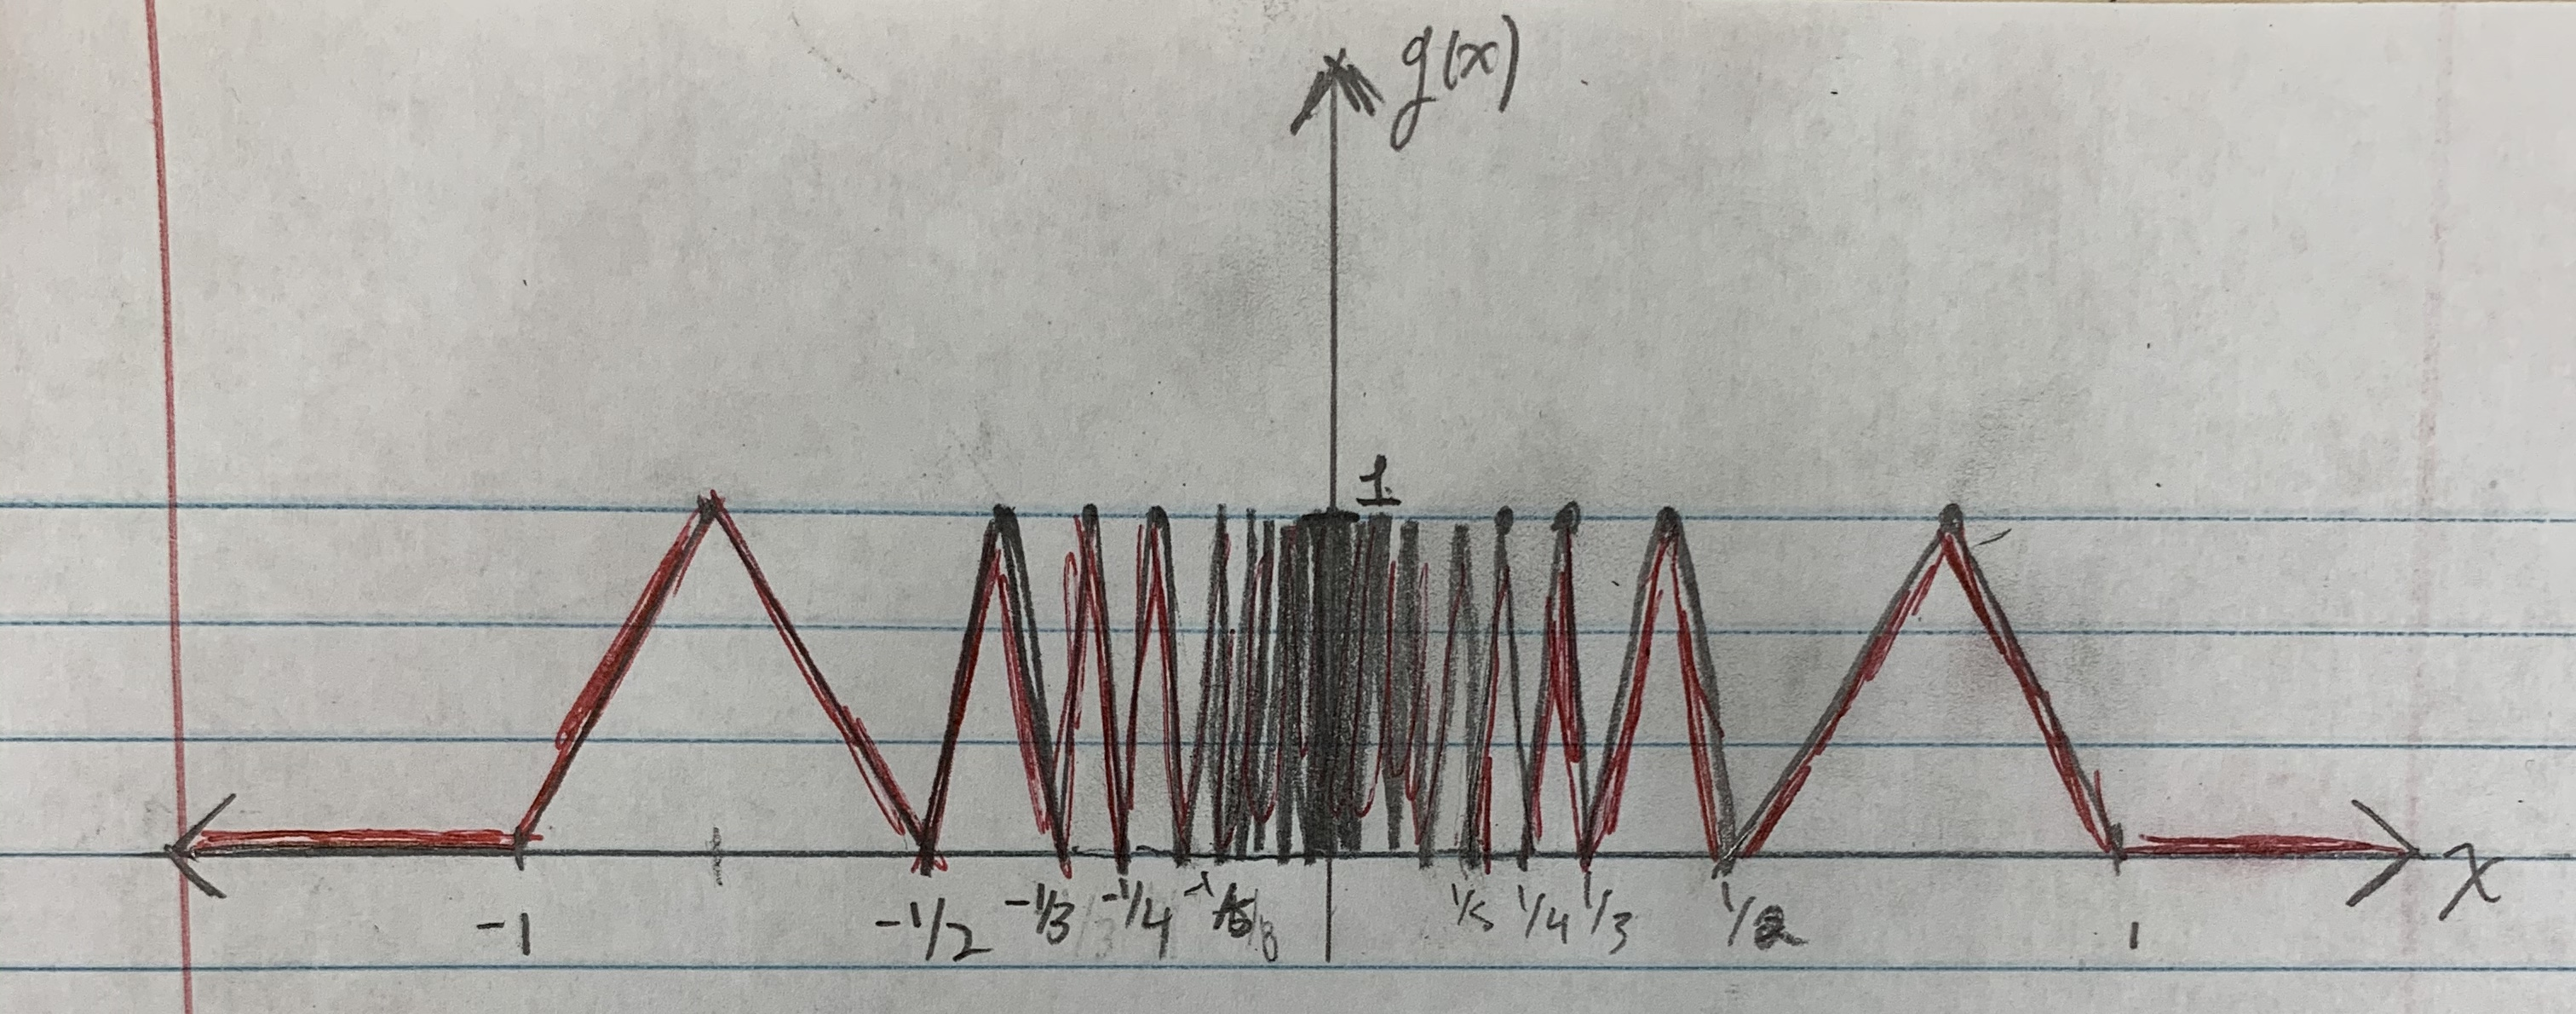
\includegraphics[width = \linewidth]{function_g.jpg}
\label{$g(x)$}
\end{figure}

Then $g$ is defined for all real numbers and $g(x) = f(x)$ for $x \in F$ (that is, $g\rvert_F = f$). So $g$ is an extension of $f$ to $\mathbb{R}$. Also, $g$ is continuous on $I_1$ and $I_2$ as $g$ is identically 0 on these open intervals. For each finite open interval $I_n = (a_n,b_n)$, $g$ is an increasing linear function on $(a_n, a_n + \frac{b_n-a_n}{2})$ and a decreasing linear function on $(a_n +\frac{b_n-a_n}{2}, b_n)$. Also, at the midpoint of each $(a_n,b_n)$, $a_n + \frac{b_n-a_n}{2}$,

$$1- \frac{2}{b_n-a_n}\left(a_n + \frac{b_n-a_n}{2} - \left(a_n + \frac{b_n-a_n}{2}\right)\right) = 1- \frac{2}{b_n-a_n}(0) = 1$$
$$\frac{2}{b_n-a_n}\left(a_n + \frac{b_n-a_n}{2} - a_n\right) = \frac{2}{b_n-a_n}\frac{b_n-a_n}{2}  = 1 \;.$$

So indeed the two lines used to define $g$ within any $I_n = (a_n,b_n)$ agree at a maximum of 1 at the midpoint of the interval. Therefore $g$ is continuous on each $I_n$. Also, at each endpoint $a_n$ and each endpoint $b_n$, we have
$$\text{lim}_{x \rightarrow a_n^+} g(x) = \text{lim}_{x\rightarrow a_n^+} \frac{2}{b_n - a_n}(x-a_n) = 0$$
$$ \text{lim}_{x\rightarrow b_n^-} g(x) = \text{lim}_{x\rightarrow b_n^-} 1 - \frac{2}{b_n - a_n}\left(x- (a_n + \frac{b_n-a_n}{2})\right) = 0 \;.$$

Since each $a_n,b_n \in F$ and $g(a_n) = g(b_n) = 0$, this shows that $g$ is continuous at each endpoint (recall also that $g \equiv 0$ on $(-\infty,-1)$ and $(1,\infty)$). Therefore, $g$ is continuous on $\overline{I_n}$ for each interval $I_n$ (this would only be an issue if we need to define $g$ on $\overline{R}$ for the case of $\overline{I_1}$, $\overline{I_2}$ but  this cannot be necessary since we are asked to find $g: \mathbb{R} \rightarrow \mathbb{R}$). As we proved in Homework 4, "$g$ is continuous on $\overline{I_n} \implies g\rvert_{\overline{I_n}}$ is continuous". \\

However, $g$ is not continuous at 0. Since $0 \in F$, $g(0) = f(0) = 0$. Consider $\epsilon = 1>0$ and let $\delta >0$ be arbitrary. Then there is a $k \in \mathbb{N}$ such that $k$ is even and  $k > 2/\delta + 2 \implies 0< 1/(k/2)< 1/(k/2 - 1) < \delta$. Thus we have an interval $I_k = \left(\frac{1}{k/2}, \frac{1}{k/2 - 1}\right) \subset (0,\delta)$ (we have $I_k = I_n= (a_n,b_n)$ for some $n$ but now it is more convenient to revert to the original notation). But then for the midpoint of this interval, $\alpha_k = 2/k + \frac{1}{2}\left(\frac{1}{k/2 - 1} - \frac{1}{k/2}\right)$, $g(\alpha_k)= 1$ using our definition of $g$. Therefore, there is an $\epsilon > 0$ (specifically $\epsilon = 1$) such that for every $\delta > 0$, we can find an $x$ ($\alpha_k$) such that $|x - 0| < \delta$ but $|g(x) - g(0)| = |1-0| = 1 \geq \epsilon$. Therefore $g$ is not continuous at $0$.\\

\end{document}